\begin{figure*}[t]
\centering
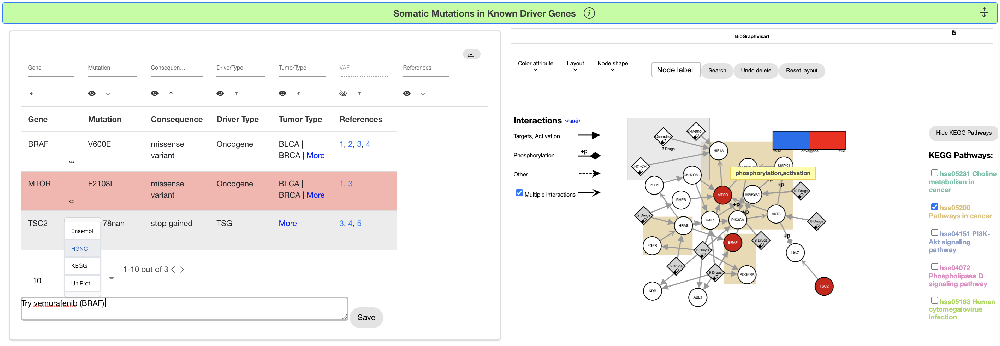
\includegraphics[width=\textwidth]{figures/system-examples/pecax_variant_network.pdf}
\caption{PeCaX connects annotated patient variants with gene--drug network context. The table summarizes somatic mutations in known driver genes, including predicted consequences, driver types, and reference sources; the associated network places affected genes alongside interacting genes and drugs, with controls for inspecting pathway context. Algorithmic annotation and network construction provide evidence that scientists can inspect when interpreting molecular findings. Cropped from Fig.~2 (upper table--network pair) in Additional file~1 of Figaschewski et al.~\cite{AnchorPeCaX}. \copyright{} The Author(s) 2023, licensed under CC BY 4.0 (\protect\url{https://creativecommons.org/licenses/by/4.0/}); cropping only.}
\label{fig:pecax-variant-network}
\end{figure*}
